\documentclass[../../main.tex]{subfiles}

% 

\begin{document}
\chapter{Charakteristiky jadrových stavov}
Aby sme boli dôsledný, tak uvedieme vlastnosti jadier, ktoré už boli spomenuté v predchádzajúcich otázkach a následne k ním pridáme aj vlastnosti, ktoré ešte neboli spomenuté.
\section{Náboj a notácia}
Náboj jadra je len súčtom protónových nábojov pretože experimentálne určený náboj neutrónu je menší ako $2\times 10^{-21}$. Neutrón však má magnetický moment. V klasickom obraze, v ktorom sú magnetické efekty spôsobené pohyblivými nábojmi, to znamená, že vo vnútri neutrónu prúdia prúdy, ale celkový náboj je nulový. Toto možno považovať za jednoduchú indikáciu toho, že neutrón je zložený objekt a nie elementárnou časticou.
\begin{itemize}
	\item Izotopy majú rovnaké protónové číslo $Z$ ale rozdielne neutrónové číslo $N$.
	\item Izobary majú rovnaké nukleónové číslo $A$.
	\item Izotóny majú rovnaké neutrónové číslo $N$ ale rozdielne protónové číslo $Z$.
	\item Jadra majú bohaté spektrum excitovaných stavov (až na pár výnimiek), ktoré sa môžu deexcitovať na základný stav emitovaním fotónov.
	\item Energetické levely jadier sú charakterizované kvantovými číslami, ktoré korešpondujú s vlastnými hodnotami operátorov. Tieto operátory komutujú s hamiltonovým operátorom jadra.
\end{itemize}

\section{Polomer atómových jadier}
Experimenty ukazujú, že atómové jadro nie je ostro ohraničene, ale že sa hustota jadrovej hmoty mení na povrchu jadra síce rýchlo, ale nie skokom. Existuje teda určitá prechodová oblasť (viď obrázok \ref{js10:polomer1}).
\begin{figure}[h]
 \centerline{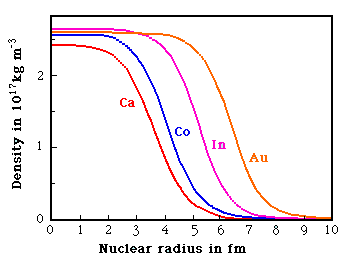
\includegraphics[width=0.5\textwidth]{js10-polomer1.png}}
 \caption{Rozdelenie hustoty pre niektoré jadrá založené na meraniach Hofstadtera et al.}
 \label{js10:polomer1}
\end{figure}
\newline
Zároveň se však ukazuje, že v bezprostrednej blízkosti jadra pôsobia na jadrové častice špecifické príťažlivé síly - jadrové síly, ktoré pre nabité častice mnohonásobne prevyšujú coulombovské síly. Je preto rozumné definovať polomer jadra ako polomer oblasti, v ktorej hrajú jadrové síly rozhodujúcu úlohu. K tomu účelu je vhodné popísať interakciu častice s jadrom pomocou potenciálu $U(r)$, o ktorom budeme predpokladať, že je sférické (čo ale v skutočnosti nie je), čo dobre aproximuje chovanie väčšiny jadier. Výsledný potenciál bude súčtom potenciálu interakcie coulombovskej $U_c(r)$ a interakcie jadrovej $U_j(r)$ 
\begin{equation} 
U(r)=U_c(r)+U_j(r).
\end{equation}
Za polomer jadra $R$ môžme potom považovať oblasť, v ktorej platí $U_c < U_j$. Schematicky je situácia znázornená na obrázku \ref{js10:polomer2}, kde v pravej časti je zachytený priebeh potenciálu $U(r)$ pre kladnú nabitú časticu. V oblasti I prevláda odpudivá coulombovská interakcia, v oblasti II jadrová interakcia. Priesečník potenciálu U s osou r udáva polomer R, ktorý môžme považovať za polomer jadra.
\begin{figure}[h]
 \centerline{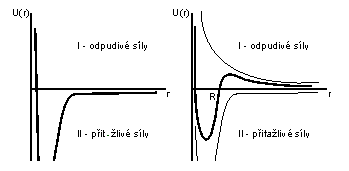
\includegraphics[width=0.5\textwidth]{js10-polomer2.png}}
 \caption{Priebeh potenciálu pre neutrón (vľavo) a protón (vpravo) v poli jadra.}
 \label{js10:polomer2}
\end{figure}
\newline
Prvé informácie o rozmere jadier boli získané na základe Rutherfodovho experimentu, kedy Rutherford ukázal, že pri prechode $\alpha$-častíc vo vzdialenosti $L=10-14\,m$ od jadra atómu dochádza k narušeniu coulombovskej interakcie. Súčasné výskumy ukazujú, že pre polomer jadier platí dostatočne presný vzťah
$$ R=r_0A^{1/3},$$
kde A je hmotnostní číslo jadra. Hodnota parametru $r_0$ je $r_0=1,3\times10^{-15}\,m$. Z tohoto vzťahu plynie dôležitý záver. Objem jadra je priamo úmerný hmotnostnému číslu A a teda každý nukleón zaberá v jadre rovnaký objem. Jadro sa teda dá približne interpretovať ako sústava nukleónov s konštantnou hustotou jadrovej hmoty. Vhodná parametrická forma jadrovej hustoty bola navrhnutá Woodom a Saxonom a má takýto tvar
$$ \rho_N(r)=\frac{\rho_0}{1+e^{\frac{r-R_N}{t}}},$$
kde $t$ je parameter hrúbky povrchu. To je vlastne zobrazene na obrázku \ref{js10:polomer1}.
\section{Hmotnosť atómových jadier}
Hmotnosť jadra je menšia ako súčet hmotností základných nukleónov. Toto odráža skutočnosť, že jadro je viazaný stav častíc. Toto vedie k definícii väzbovej energie $E_B$ jadra ako $$  M(A,Z)c^2=Zm_pc^2+(A-Z)m_nc^2-E_B.$$
\section{Väzbová energia jadra}
Väzbová energia je najlepšie popísaná Weizsäckerovou formulou vychádzajúcou z Kvapkového modelu jadra, ktorá má nasledujúci tvar
$$ E_B=b_vA-b_fA^{2/3}-b_c\frac{Z^2}{A^{1/3}}-b_a\frac{(N-Z)^2}{A}+b_p\delta A^{-3/4},$$
kde $b_v$ a $b_f$ sú objemový a povrchový člen, ktorý je spojený s tým, že pôsobenie nukleónov vo vnútri objemu jadra a na povrchu jadra je rôzne. $b_c$ je coulombovský člen pretože protóny v jadre sa navzájom odpudzujú a to zoslabuje väzbovú energiu jadra. V jadre môže ešte nastať asymetria medzi počtom protónov a neutrónov, ktorá taktiež zoslabuje väzbovú energiu. $b_p$ vyjadruje empiricky fakt, ze jadra sú silnejšie/slabšie viazane, ak ich počet protónov alebo neutrónov (alebo oboch) je párny/nepárny. Odpudzovanie alebo priťahovanie má na starosti $\delta$ člen, ktorý nadobúda nasledujúce hodnoty:
\begin{itemize}
	\item $\delta=1$ pre even-even jadro
	\item $\delta=0$ pre even-odd jadro
	\item $\delta=-1$ pre odd-odd jadro
\end{itemize}
Posledne dva členy väzbovej energie vychádzajú zo Shell modelu jadra. Na obrázku \ref{js10:prispevky} sú graficky znázornene jednotlive príspevky.
 
Tieto konštanty boli stanovené empiricky. S týmito 5 konštantami môžme určiť väzbovú energiu pre viac ako 2000 jadier s presnosťou $1-2\%$. Priemerná väzbová energia na jeden nukleón je 
$$ \epsilon=\frac{E_B}{A}.$$
Pre názornejšie grafické znázornenie pozri obrázok \ref{js10:vazby}.
\begin{figure}[h]
\begin{subfigure}[b]{0.45\textwidth}
\centering
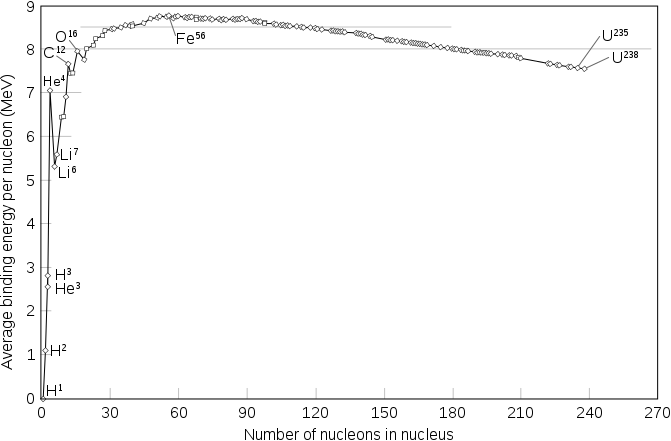
\includegraphics[width=1.0\textwidth]{js10-vazba1.png}
\end{subfigure}
\begin{subfigure}[b]{0.45\textwidth}
\centering
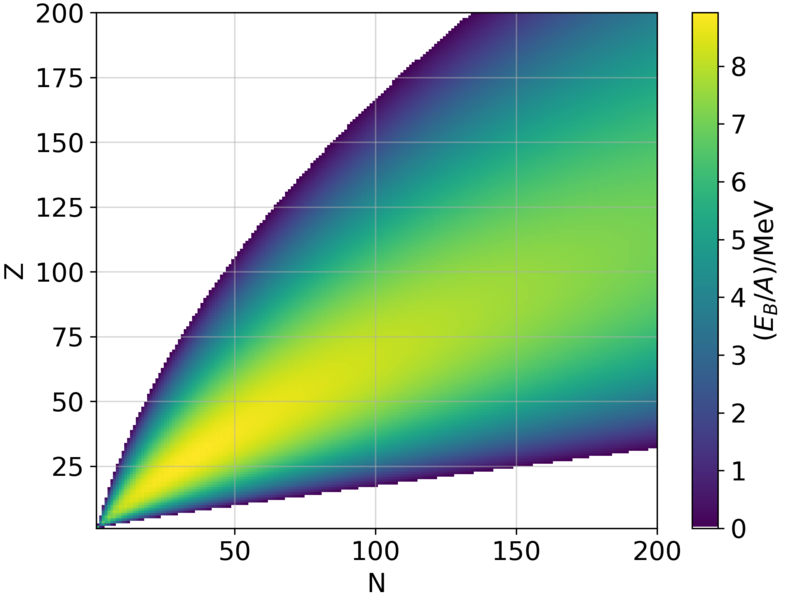
\includegraphics[width=1.0\textwidth]{js10-vazba2.png}
\end{subfigure}
\caption{\textbf{Naľavo:} Krivka väzbovej energie - bežné izotopy. \textbf{Napravo:} Grafické znázornenie semi-empirickej väzbovej energie. Väzbová energia na nukleón v MeV (najvyššie hodnoty sú žltou, viac ako 8,5 MeV na nukleón) je vynesená pre rôzne nuklidy ako funkcia atómového čísla $Z$ (os $y$) počtu neutrónov $N$ (os $x$). Najvyššie hodnoty sú zaznamenané pre $Z=26$ (železo).}
\label{js10:vazby}
\end{figure}
\begin{figure}[h]
 \centerline{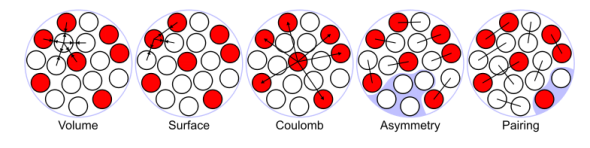
\includegraphics[width=0.8\textwidth]{js10-prispevky.png}}
 \caption{Jednotlivé príspevky väzbovej energie.}
 \label{js10:prispevky}
\end{figure}

\section{Parita, moment hybnosti, spin a celkový moment hybnosti}
Jadro je izolovaný systém a tak má dobre definovaný celkový moment hybnosti ($\vec{J}$), ktorý je definovaný ako súčet individuálnych uhlových momentov ($\vec{l}$) a spinových momentov ($\vec{s}$)
\begin{equation}
\vec{J}=\sum_{i=1}^{A}(\vec{l}_i+\vec{s}_i) 
\end{equation}
Tento vektor je jeden zo základných charakteristických vlastnosti jadrového stavu. Je potrebné mať na pamäti, že orbitálny moment hybnosti je celočíselným násobkom Planckovej konštanty, zatiaľ čo vnútorný spin nukleónov je polo-číselný násobok Planckovej konštanty (lebo protóny a neutróny sú fermióny). Takže párne jadrá majú celočíselné hodnoty pre celkový moment hybnosti a nepárne jadra majú polo-číselné hodnoty celkového momentu hybnosti. Všetky jadrá s párnym Z a párnym N majú nulový celkový moment hybnosti, $\vec{J}=0$. Celkový moment hybnosti je invariantný vzhľadom na rotáciu.

Pripomeňme, že parita je spojená s kvantovým číslom $\pm1$, čo je spojené s inverziou priestoru. To znamená, že ak $\Pi$ je operator parity, ktorý pôsobí na kompozitnú vlnovú funkciu jadra $\Psi(\vec{x},A,Z)$
potom 
\begin{equation}
\Pi \Psi(\vec{x},A,Z)=\pm \Psi(-\vec{x},A,Z).
\end{equation}
Znamienko plus je spojené s párnou funkciou a znamienko mínus je spojené so nepárnou funkciou. Celkový moment hybnosti a parita sú merateľné. Na popis sa používa notácia $J^{\Pi}$. Napríklad: $^{235}U$ má $J^{\Pi}=\frac{7}{2}^{-}$, zatiaľ čo $^{238}U$ má $J^{\Pi}=0^{+}$. Na obrázku \ref{js10:spiny} môžme vidieť príklad diskrétnych energetických hladín, ktoré sú definované kvantovými číslami (celkovým momentom hybnosti, paritou etc.)
\begin{figure}[h]
 \centerline{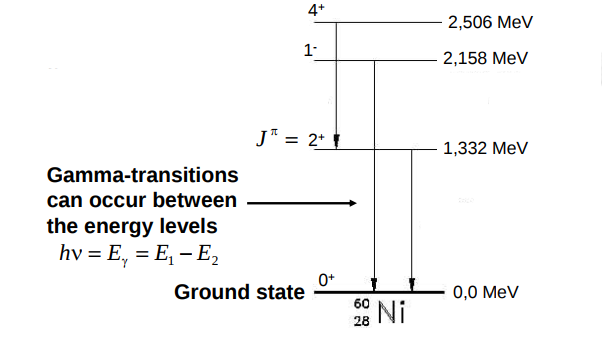
\includegraphics[width=0.6\textwidth]{js10-parita.png}}
 \caption{Energetické levely jadra $_{28}^{60}Ni$ .}
 \label{js10:spiny}
\end{figure}
\newline
Parita je daná $\Pi=-1^{(l)}$, kde $l$ je súčet jednotlivých klasických momentov hybnosti (bacha nie je to celkový moment hybnosti ani spin).
\section{Jadrový elektrický a magnetický moment}
Statické elektromagnetické vlastnosti jadier sú špecifikované pomocou elektromagnetických momentov, ktoré poskytujú informácie o tom, ako je magnetický moment a náboj distribuovaný v celom jadre. Dva najdôležitejšie momenty sú elektricky kvadrupólový moment (Q) a magnetický dipólový moment ($\mu$), ktoré si teraz predstavíme bližšie.
\subsection{Magnetický dipólový moment jadra}
Vieme, že magnetické polia generované pohyblivými nábojmi majú malý, ale merateľný účinok na energetické hladiny viazaných elektrónov v atóme. Samotné jadro je tvorené protónmi a neutrónmi, ktoré majú svoj vlastný vnútorný spin. Vďaka tomuto spinu si protóny a neutróny vytvárajú svoje vlastné spinové magnetické polia, okrem orbitálnych. To poskytuje dodatočný krútiaci moment na elektrónové spiny, čo vedie k hyperjemnej štruktúre atómových energetických hladín. Tieto energetické rozdiely sú malé ale napriek tomu dôležité pre interpretáciu atómových spektier a preto je dôležite popísať magnetické polia generované protónmi a neutrónmi. Preto sa teraz sústreďme na nukleóny v pevne viazanom jadre, kde sa tieto nukleóny pohybujú rýchlosťou približne $0,001-0,1\,c$.

Jadrové magnetické dipólové momenty vychádzajú z vnútorných spinových magnetických dipólových momentov protónov a neutrónov v jadre a z prúdov cirkulujúcich v jadre kvôli pohybu protónov. Aby sme určili príspevok orbitálneho momentu hybnosti do magnetického momentu budeme nukleóny považovať za bodové častice. Pre bodovú časticu môžme písať 
\begin{equation}
M2=\vec{\mu}=\frac{\mu_N}{\hbar}\sum_{i=1}^A\big( g_l\vec{l_i} + g_s\vec{s_i} \big),
\end{equation}
kde $\mu_N=\frac{e\hbar}{2m_p}\approx5.0507\times 10^{-27}J/T$ je jadrový magnetón, $g_l$ je g-faktor ($g_l=1$ pre protón a $g_l=0$ pre neutrón, keďže neutrón je neutrálny) a $g_s$ je spinový $g-faktor$ ($g_s=5.5856...$ pre protón, $g_s=-3.8260...$ pre neutrón a $g_s=-2.0023...$ pre elektron). Elektrónový $g-faktor$ bol veľmi presne predpovedaný z $QED$, čo vlastne bol veľký triumf tejto kvantovej teórie poľa.
\subsection{Elektrický kvadrupólový moment jadra}
Závisí od rozloženia náboja vo vnútri jadra a je mierou jadrového tvaru. Elektrostatický potenciál jadra je daný nasledovne
\begin{equation}
V(\vec{r})=\frac{1}{4\pi\epsilon_0}\int d\vec{r}^{\prime}\frac{\rho_p({\vec{r}^{\prime}})}{\lvert \vec{r}-\vec{r}^{\prime} \rvert},
\end{equation}
kde 
\begin{equation}
\int \rho_p(\vec{r}^{\prime})d\vec{r}^{\prime}=Ze
\end{equation}
Teraz si predstavme, že skúmame jadro z veľkej vzdialenosti ($r^{\prime} <<< r$), pozri obrázok \ref{js10:potencial}. 
\begin{figure}
 \centerline{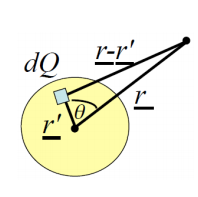
\includegraphics[width=0.2\textwidth]{js10-potenial.png}}
 \caption{Vzájomná poloha vektorov $\vec{r}^{\prime}$ a $\vec{r}$.}
 \label{js10:potencial}
\end{figure}
Za týchto okolnosti môžme daný potenciál rozvinúť pomocou Taylorovho radu v mocninách $r^{\prime}/r:$
\begin{equation}
V(r)=\frac{1}{4\pi\epsilon_0r} \big[ Ze+\frac{1}{r}\int z \rho(r^{\prime})d\vec{r}^{\prime}+\frac{1}{2r^2}\int(3z^2-r^{\prime2})\rho(r^{\prime})d\vec{r}^{\prime} +... \big] \hspace{0.7cm} kde \hspace{0.7cm} z=r^{\prime}\cos(\theta)
\end{equation}
Z kvantovej mechaniky ďalej vieme, že $ \rho(r^{\prime})=Ze [\psi(\vec{r}^{\prime})\psi^{*}(\vec{r}^{\prime})] $. Elektrické momenty sa označujú podľa mocniny $1/r$ v zátvorke
\begin{itemize}
	\item \textbf{E0 moment}: elektricky monopol (náboj) $\rightarrow$ $Ze\int \psi^{*}\psi d\vec{r}^{\prime}=Ze$.
	\item \textbf{E1 moment}: elektricky dipól $\rightarrow$ $d=\int \psi^{*}z\psi d\vec{r}^{\prime}$ $\rightarrow$. Ak bude elektrický náboj v jadre rozložený symetricky, môžme očakávať, že dipólový moment jadra bude nulový alebo veľmi veľmi malý. Experimenty ukazujú, že pre základný stav jadra je $d=0$, a teda elektrický náboj v jadre je rozložený rovnomerne. Navyše jadrové vlnové funkcie majú definovanú paritu ako $\lvert \psi(\vec{r}) \rvert^2 = \lvert \psi(-\vec{r}) \rvert^2 \Rightarrow$ elektricky dipólový moment je vždy nulový.
	\item \textbf{E2 moment}: elektricky kvadrupólový moment $\rightarrow$ $Q=\frac{1}{e} \int (3z^2-r^2)\rho(\vec{r})d\vec{r}$ $\rightarrow$ $Q$ udáva odchýlku skutočného rozloženia náboja od sférického. Elektrický quadrupólový moment jadra opisuje efektívny tvar elipsoidu rozloženia jadrového náboja. Nenulový kvadrupólový moment $Q$ naznačuje, že distribúcia náboja nie je sféricky symetrická. Prvýkrát sa objavil v deuteróne pri pozorovaní \textit{hyperjemnej} štruktúry atómových spektrálnych čiar. Všetky $J=0$ majú $Q=0$. Ak to ale nie je nulové môžu nastať dva prípady, ktoré sú znázornene na obrázku \ref{js10:kvadr}
	\begin{figure}[!h]
 	\centerline{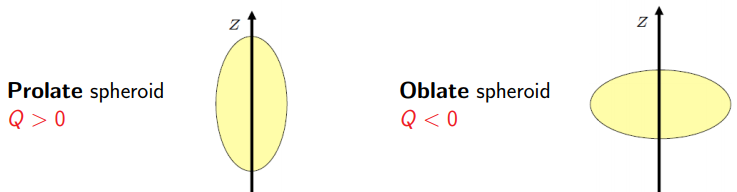
\includegraphics[width=0.8\textwidth]{js10-kvadrupol.png}}
	\caption{Grafické znázornenie kvadrupólového momentu.}
 	\label{js10:kvadr}
	\end{figure}
\end{itemize}

Interakčná energia elektromagnetickej interakcie v jadre je daná elektrickými nábojmi hadrónov a ich elektrickými prúdmi (daný pohybom nabitých hadrónov (protónov) a magnetickými momentmi hadrónov (protónov aj neutrónov). Tvar hamiltoniánu, ktorý popisuje danú interakciu je nasledovný
\begin{equation}
H_{elmag}=\int\rho(\vec{r},t)\varphi(\vec{r},t)d\vec{r}-\frac{1}{c}\int\vec{j}(\vec{r},t)\vec{A}(\vec{r},t)d\vec{r},
\end{equation}
kde $\big[ \varphi(\vec{r},t),\vec{A}(\vec{r},t) \big]$ je štvorvektor elektromagnetického potenciálu a $\big[\rho(\vec{r},t),\frac{\vec{j}}{c}(\vec{r},t)) \big]$ je štvorvektor nábojového prúdu.

Za predpokladu, že jadro budeme brat ako systém bodových nukleónov môžme písať 
\begin{itemize}
	\item hustota náboja: $\rho(\vec{r})=\sum_{i=1}^Ae\big( \frac{1}{2}+t_z^i \big)\delta(\vec{r}-\vec{r}_{i})$
	\item hustota prúdu: $\vec{j}(\vec{r})=\sum_{i=1}^Ae\big( \frac{1}{2}+t_z^i \big) \frac{1}{2}\big[\vec{v}_i \delta(\vec{r}-\vec{r}_i) + \delta(\vec{r}-\vec{r}_i)\vec{v}_i \big] + \mu_jc\sum_{i=1}^Ag_s^i(\nabla \times \vec{s}_i) \delta(\vec{r}-\vec{r}_i),$
\end{itemize}
kde $\mu_j$ je jadrový magnetón, a $t_z^i$ je projekcia izospinu (pre protón: $1/2$, pre neutrón: $-1/2$) a $g_s^i$ je gyromagnetický pomer alebo inak g-faktor, ktorý je vyjadrený nasledovne
$$ g_s^i = \frac{1}{2}g_0-t_z^ig_1 \hspace{0.5cm} kde \hspace{0.5cm} g_0=g_p+g_n \hspace{0.5cm} a \hspace{0.5cm} g_1=g_p-g_n $$

Prvý člen v hustote prúdu vznika vďaka pohybu nabitých nukleónov, zatiaľ čo druhý člen vzniká pri interakcii magnetických momentov nukleónov. Štúdiom elektromagnetickej interakcie nukleónov môžme študovať rozloženie náboja v jadre, rýchlosť, spin alebo izospin nukleónov.

Elektromagnetická konštanta jemnej štruktúry je $\alpha=1/137$. To, že je taka mala nám umožňuje použiť poruchové metódy $\Rightarrow$ zákony zachovania alebo výberove pravidla. Predpokladajme, že máme prípad, kde $\varphi=0$ a pole $\vec{A}(\vec{r},t)$ bude spĺňať Maxwelové rovnice. Spravíme multipólový rozvoj a zavedieme nejaké výberové pravidlo.

Všeobecne platí, že každé vektorové pole sa dá vyjadriť ľubovoľným úplným systémom ortogonálnych riešení Maxwelových rovníc. Po nejakých úpravách môžme ľubovolne vektorové pole vyjadriť ako 
\begin{equation}
A(\vec{r},t) = \sum_{J,M,P}dkq_k^{JMP}e^{-i\omega t}A_{JM}^P(k,r), 
\end{equation}
kde $P=E$ alebo $P=M$.

\textbf{Elektromagnetické prechody a výberové pravidlá}\par
Vďaka príspevkom od elektrických alebo magnetických momentov sú energetické hladiny jadra rozvetvene. Ako to už býva zvykom aj tu dochádza k tomu, že jadro prechádza do nižších stavov a tým emituje energiu vo forme gama žiarenia. Prechody medzi energetickými hladinami, ktoré sú spôsobené práve týmito elektromagnetickými momentami, sa nazývajú elektromagnetické prechody. Vo všeobecnosti, elektrické (náboj)
žiarenie alebo magnetické (prúd, magneticky moment) žiarenie môže byť klasifikované do multipólov $E\lambda$ alebo $M\lambda$ radu $2^{\lambda}$ ($E1\rightarrow$ elektricky dipól lebo $2^1$). Prechod, kde sa moment hybnosti počiatočného a koncového stavu zmení, môže nastať prostredníctvom niekoľkých multipólových prechodov. Najpravdepodobnejšie sa však realizujú najnižšie multipólové prechody ($E1,E2$) alebo ($M1,M2$). Emitovaná častica odnesie moment hybnosti $\lambda$, pre fotón musí platiť, že $\lambda\geq1$, keďže je to vektorová častica ($J^{\Pi}=1^{-}$). Preto prechody $E0$, $M0$ nemôžu nastať (navyše magneticky monopol ani neexistuje). Celkový moment hybnosti sa musí zachovávať a preto pre $\lambda$ musí platiť nasledovné
$$ \lvert J_i-J_f \rvert \leq \lambda \leq J_i+J_f $$
$$ J_i=J_f+\lambda,$$
navyše pre paritu musí platiť:
\begin{itemize}
	\item Pre elektrický multipólový prechod $\Pi(E\lambda)=\Pi_i\Pi_f=(-1)^{\lambda}$
	\item Pre magnetický multipólový prechod $\Pi(M\lambda)=\Pi_i\Pi_f=(-1)^{\lambda+1}$
\end{itemize}
Preto sa parita nemení pre \textit{E-párne} a \textit{M-nepárne} mutipólové prechody, zatiaľ čo pre \textit{E-nepárne} a \textit{M-párne} sa parita nezachováva. Pre ukážku takýchto prechodov pozri obrázok \ref{js10:prechody}.
\begin{figure}[!h]
\centerline{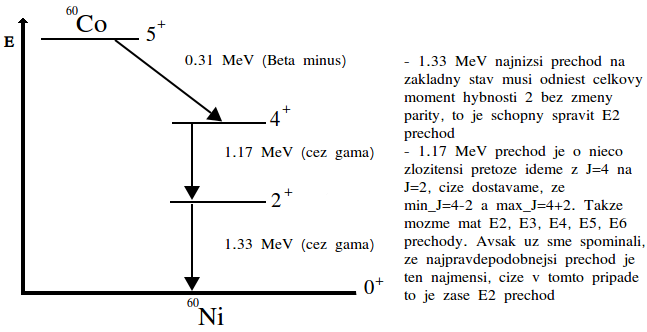
\includegraphics[width=0.9\textwidth]{js10-prechody.png}}
\caption{Schéma multipólových prechodov.}
\label{js10:prechody}
\end{figure}
\newline
Takže pre prechody medzi hladinami so spinom $J_i$ a $J_f$ a paritami $\Pi_i$ a $\Pi_j$ mame:
\begin{itemize}
	\item $J=\lvert J_i-J_f \rvert$ pre $J_i \neq J_f$.
	\item $J=1$ pre $J_i=J_f >0$
	\item Potom dostávame pravidlo: $\Pi_i\Pi_f=(-1)^{J+K}$, kde $K=0$ pre $EJ$ a $K=1$ pre $MJ$
\end{itemize}
To posledné pravidlo sme vlastne už definovali vyššie ale je dobre ho zopakovať. Navyše z tých obmedzení vidíme, že prechod s vyžiarením fotónu medzi stavmi $J_i=0$ a $J_f=0$ neexistuje.
\section{Určenie spinových hladín a multipolarity prechodu}
Na experimentálne určenie spinových hladín a multipolarity prechodu možno použiť
\begin{itemize}
	\item Využitie výberových pravidiel pre elektromagnetické prechody
	\item Využitie pomerov medzi pravdepodobnosťou gama prechodu a vyžiarenia konverzného elektrónu. Určenie konverzného koeficientu prechodu $\alpha=\frac{N_e}{N_{\gamma}}$. Jednotlive konverzné koeficienty pre jednotlivé vrstvy ($\alpha_K$, $\alpha_L$, $\alpha_M$ ...). Konverzné koeficienty rastú s nárastom multipolarity prechodu ďalej platí, že $\alpha(M)>\alpha(E)$ a tieto koeficienty rýchlo klesajú s energiou prechodu. Tieto vlastnosti možno pozorovať na obrázku \ref{js10:koef}.
	\begin{figure}[!h]
	\centerline{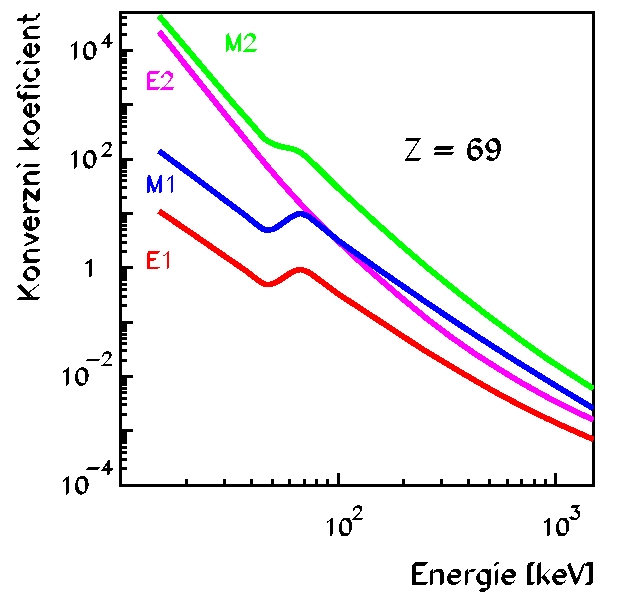
\includegraphics[width=0.4\textwidth]{js10-koenficienty.png}}
	\caption{Koeficienty prechodu.}
	\label{js10:koef}
	\end{figure}
	\item Uhlová korelácia dvoch fotónov vyžiarených za sebou v kaskáde.
	\item Údaje o spine z reakcii: analýza priebehu rôznych reakcii-rôzne reakcie budia hladiny s rôznym spinom.
\end{itemize}
\section{Určovanie pravdepodobnosti prechodu z doby života hladín}
\begin{itemize}
	\item Elektronické metódy - meranie krivky rozpadu: meranie izomerných stavov, meranie mimo zväzok ($\tau \sim min-\infty$), transportný systém a meranie behom ožarovania ($\tau > \sim s$), meranie na zväzku (celkove rozlíšenie rádovo v jednotkách až zlomkoch ns). Časové spektrum je tvorené gaussiánom $+$ exponenciálnou krivkou. Dosiahnuteľná dolná hranica $\tau \sim ns$.
	\item Využitie štúdia Dopplerovsky posunutej a neposunutej linky v závislosti na vzdialenosti, v ktorej sú odrazené jadra zastavené. Merateľná oblasť dôb života $\tau \sim 10^{-10}- 0^{-12}\,s$.
	\item Metóda zoslabenia Dopplerovho posunu energie žiarenia gama. Produckia odrazeného jadra $\rightarrow$ brzdenie a rozptyl v terči alebo v podložke $\rightarrow$ vyžiarený fotón má rôzny Dopplerov posun energie $\rightarrow$ zložitý tvar linky. Zo štúdia tvaru linky sa dá určiť doba života. Vzťah medzi ionizačnými stratami a drahou je $\Delta x=(dE/dx)^{-1}\Delta E$. Táto metóda má problémy s popisom brzdenia a mnohonásobného rozptylu odrazeného jadra. Merateľná oblasť doby života je $\tau \sim 10^{-12}-10^{-15}\,s$.
\end{itemize}
\section{Určenie pravdepodobnosti prechodu pomocou Coulombovského budenia}
Využívajú sa zväzky ťažkých iónov $\rightarrow$ vysoký náboj $\rightarrow$ budenie stavu s vysokým spinom. Energia zväzku nesmie prekonať energiu Coulombovskej bariéry $E_{CB} \sim \frac{Z_1Z_2}{A_1^{-1/3}+A_2^{-1/3}}$, kde $Z_1$, $Z_2$, $A_1$, $A_2$ sú parametre nalietavajúceho a terčového jadra. Výhody
\begin{itemize}
	\item čistý elektromagneticky proces
	\item minimálne pozadie
	\item dominantne budenie prostredníctvom $E2$ prechodu 
\end{itemize}
Merane doby života $\tau \sim 10^{13}-10^{-9}\,s$.
\section{Štúdium stavov s veľmi vysokým spinom - spiny až $ I\hbar \geq 40\hbar$}
Budenie vysoko-spinových stavov v zrážkach ťažkých iónov. Po zrážke sa vytvorí zložene jadro ($\tau > 10^{-20}\,s$) - jadra s prebytkom protónov alebo zväzky rádioaktívnych jadier (aj jadra s prebytkom neutrónov).
Excitačná energia 
$$E_{EX}=E_{CM}+Q,$$ 
kde $Q$ je energia reakcie a $E_{Cm}$ je energia projektilu v CM. Maximálny dosiahnuteľný spin je 
$$I^2_{max}=\frac{2\mu R^2}{\hbar^2}(E_{CM}-v_c),$$
kde $\mu$ je redukovaná hmotnosť a $R$ je najväčšia vzdialenosť, pri ktorej ešte vznikne zložené jadro. Štúdium týchto stavov umožňujú $4\pi$ multidetektorové spektrometre.

Po vzniku zloženého jadra sa vypari niekoľko nukleónov (prevažne neutróny, lebo sú neutrálne a tak nemusia prekonať Coulombovskú bariéru) $\rightarrow$ rýchly úbytok energie ($\sim 8\,MeV/nukleon$) ale len malý úbytok momentu ($\sim 1 \hbar/nukleon$). Týmto procesom však konkurujú vysoko-energetické gama vybíjacie gigantické dipólové rezonancie.

\begin{enumerate}
	\item Štatistický začínajú vo vysokej hustote stavov prechody $E1$.
	\item $E2$ prechody nastavajú blízko Yrast línie.
	\item Pravidelná štruktúra rotačných pásov $\sim 1\,MeV$ nad Yrast líniou $\rightarrow$ dostatočná intenzita $\rightarrow$ porovnávanie jednotlivých prechodov.
\end{enumerate}
Yrast línia - spája stavy s najväčším spinom pre danú energiu. Celková doba vybíjania $\sim 10^{-9}\,s$ s počtom vyžiarených fotónov $\sim 30$. Rozlišujeme tu dva typy rotácie 
\begin{itemize}
	\item Kolektívna rotácia - oblasť deformovaných jadier - kolektívny pohyb nukleónov.
	\item Nekolektívna rotácia - sférické a slabo deformované jadra - vysoký spin je daný pohybom niekoľkých nukleónov.
\end{itemize}
Pre vysoké spiny nastávajú prechody medzi jednotlivými druhmi rotácie a to drasticky zmení tvar jadra. Vysoké spiny $\rightarrow$ rýchla rotácia $\rightarrow$ silná Coriolisová interakcia medzi časticovým a rotačným pohybom $\rightarrow$ kríženie pásov $\rightarrow$ silná Coriolisová interakcia znižuje energiu vybudeného jedno-časticového stavu, nad ktorým je rozvinutý rotačný pás $\rightarrow$ dochádza k prekríženiu energetických pásov.
\section{Superdeformované stavy}
Stavy s veľmi vysokou deformáciou (pomer os 2:1 a viac), ktoré sú predpovedané Shell modelom. Nastávajú pre vysoké spiny $\sim 40-70 \hbar$. Dlhé rotačné pásy sú vybíjané dlhými kaskádami $E2$ prechodov.
\section{Gigantické rezonancie}
Vzájomný kolektívny pohyb rôznych typov nukleónov, pozri obrázok \ref{js10:gigant},
\begin{itemize}
	\item s rôznou orientáciou spinu
	\item s rôznou orientáciou izospinu (protónové kvapaliny voči neutrónovým kvapalinám)
\end{itemize}
Gigantické rezonancie se veľmi dobre získavajú pomocou Coulombovskej excitácie.
\begin{figure}[!h]
\centerline{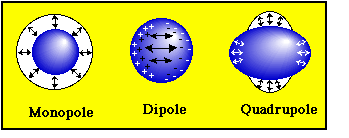
\includegraphics[width=0.5\textwidth]{js10-gignat.png}}
\caption{Rôzne typy gigantických rezonancii.}
\label{js10:gigant}
\end{figure}
Takéto typy rezonancii sú študované napríklad spektrometrom TAPS v GSI Darmstadt.

\end{document}